
% RUN:
% pdflatex -output-directory=/Users/salvatorpes/Desktop/Aprendizagem/Homework4/trash /Users/salvatorpes/Desktop/Aprendizagem/Homework4/G022.tex

% ir a settings.json e adicionar:
% // According to the wiki, the string latex-workshop.latex.autoBuild.run has three possible values: never, onSave and onFileChange(default).
% "latex-workshop.latex.autoBuild.run": "never",

\documentclass{article}


\author{Pedro Curvo (ist1102716) $|$ Salvador Torpes (ist1102474)}

\usepackage[utf8]{inputenc}
\usepackage[english]{babel}
% \usepackage[letterpaper,top=10mm,bottom=15mm,left=15mm,right=15mm,marginparwidth=1.75cm]{geometry}
% \usepackage[letterpaper,top=10mm,bottom=15mm,left=15mm,right=15mm,marginparwidth=1.75cm]{geometry}
\usepackage[letterpaper,margin=1in,marginparwidth=1.75cm]{geometry}
\usepackage{multicol}
\usepackage{biblatex}
\usepackage{cancel}
\usepackage{colortbl}
\addbibresource{Bibliografia.bib}
\usepackage{graphicx}
% \graphicspath{{../Homework1/images/}}
\usepackage{subcaption}
\usepackage{tabularx}
\usepackage{ulem}
\usepackage{booktabs}
\usepackage{array}
\usepackage{makecell}
\usepackage{multirow}
\usepackage{amsmath}
\usepackage{makecell}
\usepackage{url}
\usepackage{csquotes}
\usepackage{caption}
\usepackage{enumitem}
\usepackage{textcomp}
\usepackage{pdflscape}
\usepackage{makeidx}
\usepackage{amsmath}
% \usepackage{tocbibind}
\providecommand{\tightlist}{\relax}
\usepackage{tocloft}
\renewcommand{\cftsecindent}{0em}
\renewcommand{\cftsubsecindent}{1em}
\renewcommand{\cftsecfont}{\bfseries}
\renewcommand{\cftsubsecfont}{\itshape}
\setlength{\cftsubsecnumwidth}{0em}

\usepackage[version=4]{mhchem}
\usepackage{hyperref} % Remove "pdftex" option here
\usepackage{float}
\usepackage{fancyhdr}
\usepackage{ragged2e}
\usepackage{xkeyval}
%\usepackage{minted}
%\usemintedstyle{manni}
\usepackage{listings}
\usepackage{amssymb}




\usepackage{tikz}
\usetikzlibrary{positioning}
\usetikzlibrary{positioning, arrows.meta}
\usepackage{adjustbox}
\usepackage{sidecap}



% \usepackage[table,xcdraw]{xcolor}
\usepackage[LY1]{fontenc}
\usepackage{tikz-3dplot}
% \usepackage{pgfplots}
\usetikzlibrary{calc, 3d, arrows}
\usepackage{forest}




\usetikzlibrary{shapes.geometric, arrows}


\lstset{
    language=Python,
    basicstyle=\ttfamily,
    keywordstyle=\color{blue},
    commentstyle=\color{gray},
    stringstyle=\color{orange},
    numbers=left,
    numberstyle=\tiny,
    numbersep=5pt,
    showspaces=false,
    showstringspaces=false,
    breaklines=true,
    frame=tb,
    framexleftmargin=2em,
    xleftmargin=2em,
}


%\usepackage{fontspec}

%\setmonofont{Fira Code}

\fancyhf{}
\cfoot{\thepage}
\fancyhf{} % Clear all header and footer fields
\renewcommand{\headrulewidth}{0pt} % Remove the header rule line
\cfoot{\thepage} % Set the page number in the center of the footer

\pagestyle{fancy} % Apply the fancy page style

\setlength\columnsep{20pt}

\renewcommand{\familydefault}{\sfdefault}

\newenvironment{Figure}
  {\par\medskip\noindent\minipage{\linewidth}}
  {\endminipage\par\medskip}

\makeatletter
\newenvironment{figurehere}
{\def\@captype{figure}}
{}
\makeatother

\hypersetup{
  colorlinks,
  linkcolor=blue,
  anchorcolor=black,
  citecolor=cyan,
  filecolor=cyan,
  menucolor=cyan,
  urlcolor=cyan,
  bookmarksopen=true,
  bookmarksnumbered=true
}

\makeindex


\title{\vspace{-6mm}
\includegraphics[width=15mm,scale=2]{images/IST_Logo.png}\\ \vspace{5mm}
Machine Learning - Homework 4 \vspace{-5mm}}
\date{1st Term - 23/24}

\usepackage{sansmathfonts}
\usepackage[T1]{fontenc}
\usepackage[OT1]{fontenc}

\usepackage{listings}
\usepackage{xcolor}

\definecolor{codegreen}{rgb}{0,0.6,0}
\definecolor{codegray}{rgb}{0.5,0.5,0.5}
\definecolor{codepurple}{rgb}{0.58,0,0.82}
\definecolor{backcolour}{rgb}{0.95,0.95,0.92}

\lstdefinestyle{mystyle}{
  backgroundcolor=\color{backcolour},   
  commentstyle=\color{codegray},
  keywordstyle=\color{magenta},
  numberstyle=\tiny\color{codegray},
  stringstyle=\color{codegreen},
  keywordstyle=[2]{\color{orange}},
  keywords=[2]{plt.},
  basicstyle=\ttfamily\footnotesize,
  breakatwhitespace=false,         
  breaklines=true,                 
  captionpos=b,                    
  keepspaces=true,                 
  numbers=left,                    
  numbersep=5pt,                  
  showspaces=false,                
  showstringspaces=false,
  showtabs=false,                  
  tabsize=2,
  frame=single,
  framesep=2pt,
  framerule=0pt,
  xleftmargin=2pt,
  xrightmargin=2pt,
  aboveskip=1em,
  belowskip=1em,
  abovecaptionskip=0.5em,
  belowcaptionskip=0.5em,
  caption=\lstname,
  captionpos=b,
  language=Python,
  morekeywords={as},
  deletekeywords={None},
  emph={self},
  emphstyle=\color{blue},
  escapeinside={(*@}{@*)},
  literate={+}{{\textcolor{blue}{+}}}1
       {*}{{\textcolor{blue}{*}}}1
       {-}{{\textcolor{blue}{-}}}1
       {/}{{\textcolor{blue}{/}}}1
       {=}{{\textcolor{blue}{=}}}1
       {>}{{\textcolor{blue}{>}}}1
       {<}{{\textcolor{blue}{<}}}1
       {==}{{\textcolor{blue}{==}}}2
       {!=}{{\textcolor{blue}{!=}}}2
       {<=}{{\textcolor{blue}{<=}}}2
       {>=}{{\textcolor{blue}{>=}}}2,
  }
    
    \lstset{style=mystyle}
    \usepackage{fancyhdr}
    
    % Define header and footer styles
    \fancypagestyle{plain}{%
      \fancyhf{}% Clear header/footer
      \fancyhead[L]{Homework 4}% Header left
      \fancyhead[C]{2023/2024}% Header left
      \fancyhead[R]{Machine Learning}% Header right
      \fancyfoot[C]{\thepage}% Footer center
      \renewcommand{\headrulewidth}{0.4pt}% Header rule
      \renewcommand{\footrulewidth}{0pt}% Footer rule
    }
    
    % Apply the style to all pages except the first one
    \pagestyle{plain}
    \thispagestyle{empty} % Remove header/footer from first page


    \usepackage{amsmath} % for aligned
    %\usepackage{amssymb} % for \mathbb
    \usepackage{tikz}
    %\usepackage{etoolbox} % for \ifthen
    \usepackage{listofitems} % for \readlist to create arrays
    \usetikzlibrary{arrows.meta} % for arrow size
    \usepackage[outline]{contour} % glow around text
    \contourlength{1.4pt}

\begin{document}
    
\renewcommand{\arraystretch}{1.9}
\setlength{\columnseprule}{0.4pt}
\tdplotsetmaincoords{70}{110} % Set the viewing angle
\newcolumntype{M}[1]{>{\centering\arraybackslash\vspace{#1}}m{0.5\linewidth}<{\vspace{#1}}}
\newcolumntype{C}[2]{>{\centering\arraybackslash\vspace{#1}\rule{0pt}{#1}\hspace{0pt}}m{#2}}
\ifx\undefined\w
\newcolumntype{w}[1]{>{\centering\arraybackslash}m{#1}}
\fi
\renewcommand*\familydefault{\sfdefault} %% Only if the base font of the document is to be sans serif

\maketitle
\vspace{-5mm}
\hrulefill




\section*{Pen and Paper Exercises}

\section*{Dataset}

In the following exercise our goal is to consider a Bayesian Clustering model in order to separate the observations into 2 different clusters:

\[ x_1 = \begin{bmatrix} 1 \\ 0.6 \\ 0.1 \end{bmatrix} \qquad x_2 = \begin{bmatrix} 0 \\ -0.4 \\ 0.8 \end{bmatrix} \qquad x_3 = \begin{bmatrix} 0 \\ 0.2 \\ 0.5 \end{bmatrix} \qquad x_4 = \begin{bmatrix} 1 \\ 0.4 \\ -0.1 \end{bmatrix} \]

We are working with 3 different variables ($y_1, y_1, y_3$) for each observation. 
In addition, we are assuming:
\begin{enumerate}
  \item $\{ y_1 \} \perp \{y_2, y_3\}$
  \item $y_1$ follows a Bernoulli distribution with parameter $p$: $y_1 \sim \text{Bernoulli}(p)$
  \[ P(y_1 = 1) = p \qquad P(y_1 = 0) = 1 - p \]
  \item $y_2$ and $y_3$ follow a multivariate gaussian distribution with parameters $\vec{\mu}$ and $\Sigma$: $y_2, y_3 \sim \mathcal{N}(\vec{\mu}, \Sigma)$
  \[ P(\vec{x}) = \frac{1}{2\pi \sqrt{|\Sigma|}} \exp \left( -\frac{1}{2} (\vec{x} - \vec{\mu})^T \Sigma^{-1} (\vec{x} - \vec{\mu}) \right) \]
  \[ \vec{x} = ( y_2, y_3) \]
\end{enumerate}

\newpage

\section*{1\textsuperscript{st} Question}

\subsection*{Computing the Responsibilities}

First, we need to compute the responsibility of each cluster for each observation. The responsibility $\gamma_{ki}$ is defined as the probability of belonging to cluster $k$ for observation $i$:

\[ \gamma_{ki} = P(c_k | \vec{x}_i) =_{\text{Bayes}} \frac{P(\vec{x}_i | c_k) P(c_k)}{P(\vec{x}_i)} = \frac{P(\vec{x}_i | c_k) P(c_k)}{\sum_{j=1}^K P(\vec{x}_i | c_j) P(c_j)} \]

\[ \sum_{j=1}^K P(\vec{x}_i | c_j) P(c_j) = P(\vec{x}_i) \]

Where $c_k$ is the cluster $k$, $K$ is the number of clusters and $\vec{x}_i$ is the observation $i$. In addition, the probability of belonging to cluster $k$, $P(c_k)$, is represented by the mixing coefficient $\pi_k$:

\[ P(c_k) = \pi_k \]

In order to compute the responsibilities, we're told to use the following parameters for each cluster's $y_1$ and $y_2, y_3$ distributions:

\begin{table}[h!]
  \centering
  \begin{tabular}{c|c|c|c}
    Cluster & $\pi_k$ & Parameters for $\{y_1\}$ & Parameters for $\{y_2, y_3\}$ \\ \hline
    \rule{0pt}{30pt}
    1 ($c_1$) & $P(c_1) = \pi_1 = 0.5$ & $p_1 = P(y_1 = 1) = 0.3$ & $\{y_2, y_3\} \sim \mathcal{N}\left( \vec{\mu}_1 = \begin{bmatrix} 1 \\ 1 \end{bmatrix}, \Sigma_1 = \begin{bmatrix} 2 & 0.5 \\ 0.5 & 2 \end{bmatrix} \right)$ \\ 
    \rule{0pt}{30pt}
    2 ($c_2$) & $P(c_2) = \pi_2 = 0.5$ & $p_2 = P(y_1 = 1) = 0.7$ & $\{y_2, y_3\} \sim \mathcal{N}\left( \vec{\mu}_2 = \begin{bmatrix} 0 \\ 0 \end{bmatrix}, \Sigma_2 = \begin{bmatrix} 1.5 & 1 \\ 1 & 1.5 \end{bmatrix} \right)$ \\ 
  \end{tabular}
  \caption{Initial Parameters for each cluster}
  \label{tab:initial_parameters}
\end{table}

\subsubsection*{Responsibilities for $\vec{x}_1$}

First of all, we will compute $P(\vec{x}_1 | c_k) P(c_k)$ for clusters $c_1$ and $c_2$:

\[ P(\vec{x}_1 | c_1) P(c_1) = P(y_1 = 1 | c_1) P(\{y_2, y_3\}  = \{0.6, 0.1\} | c_1) \pi_1 = 0.3 \cdot 0.06658 \cdot 0.5 = 0.00999 \]

\[ P(\vec{x}_1 | c_2) P(c_2) = P(y_1 = 1 | c_2) P(\{y_2, y_3\}  = \{0.6, 0.1\} | c_2) \pi_2 = 0.7 \cdot 0.11962 \cdot 0.5 = 0.04187 \]

And then, we can compute $\gamma_{ki}$:

\[ \gamma_{11} = P(c_1| \vec{x}_1) = \frac{P(\vec{x}_1 | c_1) P(c_1)}{P(\vec{x}_1)} = \frac{P(\vec{x}_1 | c_1) P(c_1)}{\sum_{j=1}^2 P(\vec{x}_1 | c_j) P(c_j)} = \frac{0.00999}{0.00999 + 0.04187} = 0.19259 \]

\[ \gamma_{21} = P(c_2| \vec{x}_1) = \frac{P(\vec{x}_1 | c_2) P(c_2)}{P(\vec{x}_1)} = \frac{P(\vec{x}_1 | c_2) P(c_2)}{\sum_{j=1}^2 P(\vec{x}_1 | c_j) P(c_j)} = \frac{0.04187}{0.00999 + 0.04187} = 0.80741 \]

\subsubsection*{Responsibilities for $\vec{x}_2$}

First of all, we will compute $P(\vec{x}_2 | c_k) P(c_k)$ for clusters $c_1$ and $c_2$:

\[ P(\vec{x}_2 | c_1) P(c_1) = P(y_1 = 0 | c_1) P(\{y_2, y_3\}  = \{-0.4, 0.8\} | c_1) \pi_1 = 0.7 \cdot 0.05005 \cdot 0.5 = 0.01752 \]

\[ P(\vec{x}_2 | c_2) P(c_2) = P(y_1 = 0 | c_2) P(\{y_2, y_3\}  = \{-0.4, 0.8\} | c_2) \pi_2 = 0.3 \cdot 0.06819 \cdot 0.5 = 0.01023 \]

And then, we can compute $\gamma_{ki}$:

\[ \gamma_{12} = P(c_1| \vec{x}_2) = \frac{P(\vec{x}_2 | c_1) P(c_1)}{P(\vec{x}_2)} = \frac{P(\vec{x}_2 | c_1) P(c_1)}{\sum_{j=1}^2 P(\vec{x}_2 | c_j) P(c_j)} = \frac{0.01752}{0.01752 + 0.01023} = 0.63135 \]

\[ \gamma_{22} = P(c_2| \vec{x}_2) = \frac{P(\vec{x}_2 | c_2) P(c_2)}{P(\vec{x}_2)} = \frac{P(\vec{x}_2 | c_2) P(c_2)}{\sum_{j=1}^2 P(\vec{x}_2 | c_j) P(c_j)} = \frac{0.01023}{0.01752 + 0.01023} = 0.36865 \]

\subsubsection*{Responsibilities for $\vec{x}_3$}

First of all, we will compute $P(\vec{x}_3 | c_k) P(c_k)$ for clusters $c_1$ and $c_2$:

\[ P(\vec{x}_3 | c_1) P(c_1) = P(y_1 = 0 | c_1) P(\{y_2, y_3\}  = \{0.2, 0.5\} | c_1) \pi_1 = 0.7 \cdot 0.06837 \cdot 0.5 = 0.02393 \]

\[ P(\vec{x}_3 | c_2) P(c_2) = P(y_1 = 0 | c_2) P(\{y_2, y_3\}  = \{0.2, 0.5\} | c_2) \pi_2 = 0.3 \cdot 0.12958 \cdot 0.5 = 0.01944 \]

And then, we can compute $\gamma_{ki}$:

\[ \gamma_{13} = P(c_1| \vec{x}_3) = \frac{P(\vec{x}_3 | c_1) P(c_1)}{P(\vec{x}_3)} = \frac{P(\vec{x}_3 | c_1) P(c_1)}{\sum_{j=1}^2 P(\vec{x}_3 | c_j) P(c_j)} = \frac{0.02393}{0.02393 + 0.01944} = 0.55181 \]

\[ \gamma_{23} = P(c_2| \vec{x}_3) = \frac{P(\vec{x}_3 | c_2) P(c_2)}{P(\vec{x}_3)} = \frac{P(\vec{x}_3 | c_2) P(c_2)}{\sum_{j=1}^2 P(\vec{x}_3 | c_j) P(c_j)} = \frac{0.01944}{0.02393 + 0.01944} = 0.44819 \]

\subsubsection*{Responsibilities for $\vec{x}_4$}

First of all, we will compute $P(\vec{x}_4 | c_k) P(c_k)$ for clusters $c_1$ and $c_2$:

\[ P(\vec{x}_4 | c_1) P(c_1) = P(y_1 = 1 | c_1) P(\{y_2, y_3\}  = \{0.4, -0.1\} | c_1) \pi_1 = 0.3 \cdot 0.05905 \cdot 0.5 = 0.00886 \]

\[ P(\vec{x}_4 | c_2) P(c_2) = P(y_1 = 1 | c_2) P(\{y_2, y_3\}  = \{0.4, -0.1\} | c_2) \pi_2 = 0.7 \cdot 0.12450 \cdot 0.5 = 0.04358 \]

And then, we can compute $\gamma_{ki}$:

\[ \gamma_{14} = P(c_1| \vec{x}_4) = \frac{P(\vec{x}_4 | c_1) P(c_1)}{P(\vec{x}_4)} = \frac{P(\vec{x}_4 | c_1) P(c_1)}{\sum_{j=1}^2 P(\vec{x}_4 | c_j) P(c_j)} = \frac{0.00886}{0.00886 + 0.04358} = 0.16892 \]

\[ \gamma_{24} = P(c_2| \vec{x}_4) = \frac{P(\vec{x}_4 | c_2) P(c_2)}{P(\vec{x}_4)} = \frac{P(\vec{x}_4 | c_2) P(c_2)}{\sum_{j=1}^2 P(\vec{x}_4 | c_j) P(c_j)} = \frac{0.04358}{0.00886 + 0.04358} = 0.83108 \]

\subsubsection*{Responsibilities}

\begin{align*}
  \gamma_{11} &= 0.19259 & \gamma_{12} &= 0.63135 & \gamma_{13} &= 0.55181 & \gamma_{14} &= 0.16892 \\
  \gamma_{21} &= 0.80741 & \gamma_{22} &= 0.36865 & \gamma_{23} &= 0.44819 & \gamma_{24} &= 0.83108
\end{align*}

\subsection*{M-Step}

In the M-Step (Maximization Step), we will compute the new parameters for each cluster (we need to update the parameters in the table \ref{tab:initial_parameters}).

\subsubsection*{New Parameters for Cluster $c_1$}

\[ \vec{\mu}_{1_{\text{new}}} = \frac{\sum_{i=1}^4 \gamma_{1i} \vec{x}_i}{\sum_{i=1}^4 \gamma_{1i}} = \begin{bmatrix} 0.02651 & 0.50713  \end{bmatrix} \]

\[ \Sigma_{1_{\text{new}}} = \frac{\sum_{i=1}^4 \gamma_{1i} \left(\vec{x}_i - \vec{\mu}_{1_{\text{new}}} \right) \left( \vec{x}_i - \vec{\mu}_{1_{\text{new}}}\right)^T}{\sum_{i=1}^4 \gamma_{1i}} = \begin{bmatrix}  0.14137 & -0.10541 \\  -0.10541 &  0.09605  \end{bmatrix} \]

\[ p_{1_{\text{new}}} = \frac{\sum_{i=1}^4 \gamma_{1i} \vec{x}_i}{\sum_{i=1}^4 \gamma_{1i}} = 0.23404 \]

\[ \pi_{1_{\text{new}}} = \frac{\sum_{i=1}^4 \gamma_{1i}}{4} = 0.38617 \]

\subsubsection*{New Parameters for Cluster $c_2$}

\[ \vec{\mu}_{2_{\text{new}}} = \frac{\sum_{i=1}^4 \gamma_{2i} \vec{x}_i}{\sum_{i=1}^4 \gamma_{2i}} = \begin{bmatrix} 0.30914 & 0.21042  \end{bmatrix} \]

\[ \Sigma_{2_{\text{new}}} = \frac{\sum_{i=1}^4 \gamma_{2i} \left(\vec{x}_i - \vec{\mu}_{2_{\text{new}}} \right) \left( \vec{x}_i - \vec{\mu}_{2_{\text{new}}}\right)^T}{\sum_{i=1}^4 \gamma_{2i}} = \begin{bmatrix}  0.10829 & -0.08865 \\  -0.08865 &  0.10412  \end{bmatrix} \]

\[ p_{2_{\text{new}}} = \frac{\sum_{i=1}^4 \gamma_{2i} \vec{x}_i}{\sum_{i=1}^4 \gamma_{2i}} = 0.66732 \]

\[ \pi_{2_{\text{new}}} = \frac{\sum_{i=1}^4 \gamma_{2i}}{4} = 0.61383 \]

\subsection*{New table with the updated parameters}

\begin{table}[h!]
  \centering
  \begin{tabular}{c|c|c|c}
    Cluster & $\pi_k$ & Parameters for $\{y_1\}$ & Parameters for $\{y_2, y_3\}$ \\ \hline
    \rule{0pt}{30pt}
    1 ($c_1$) & $\pi_1 = 0.38617$ & $p_1 = 0.23404$ & $\{y_2, y_3\} \sim \mathcal{N}\left( \vec{\mu}_1 = \begin{bmatrix} 0.02651 \\ 0.50713 \end{bmatrix}, \Sigma_1 = \begin{bmatrix} 0.14137 & -0.10541 \\ -0.10541 & 0.09605 \end{bmatrix} \right)$ \\ 
    \rule{0pt}{30pt}
    2 ($c_2$) & $\pi_2 = 0.61383$ & $p_2 = 0.66732$ & $\{y_2, y_3\} \sim \mathcal{N}\left( \vec{\mu}_2 = \begin{bmatrix} 0.30914 \\ 0.21042 \end{bmatrix}, \Sigma_2 = \begin{bmatrix} 0.10829 & -0.08865 \\ -0.08865 & 0.10412 \end{bmatrix} \right)$ \\ 
  \end{tabular}
  \caption{New Parameters for each cluster}
  \label{tab:new_parameters}
\end{table}

\newpage

\section*{2\textsuperscript{nd} Question}

We now have a new observation $\vec{x}_{\text{new}}$ and want to compute the probability of belonging to each cluster. The new observation is:

\[ \vec{x}_{\text{new}} = \begin{bmatrix} 1 \\ 0.3 \\ 0.7 \end{bmatrix} \]

First, we will compute $P(\vec{x}_{\text{new}} | c_k) P(c_k)$ for clusters $c_1$ and $c_2$:

\[ P(\vec{x}_{\text{new}} | c_1)P(c_1)= P(y_1 = 1 | c_1) P(\{y_2, y_3\}   = \{0.3, 0.7\} | c_1) \cdot \pi_1 = 0.23404 \cdot 0.02708 \cdot 0.38617 = 0.00245 \]

\[ P(\vec{x}_{\text{new}} | c_2)P(c_2) = P(y_1 = 1 | c_2) P(\{y_2, y_3\}   = \{0.3, 0.7\} | c_2) \cdot \pi_2 = 0.66732 \cdot 0.06843 \cdot 0.61383 = 0.02803 \]

And then, we can compute $\gamma_{ki}$:

\[ \gamma_{1_{\text{new}}} = P(c_1| \vec{x}_{\text{new}}) = \frac{P(\vec{x}_{\text{new}} | c_1) P(c_1)}{P(\vec{x}_{\text{new}})} = \frac{0.00245}{0.00245 + 0.02803} = 0.08029 \]

\[ \gamma_{2_{\text{new}}} = P(c_2| \vec{x}_{\text{new}}) = \frac{P(\vec{x}_{\text{new}} | c_2) P(c_2)}{P(\vec{x}_{\text{new}})} = \frac{0.02803}{0.00245 + 0.02803} = 0.91971 \]

\paragraph{Answer} We can conclude that the observation $\vec{x}_{\text{new}}$ belongs to cluster $c_2$ with a probability of 0.91971 and to cluster $c_1$ with a probability of 0.08029.

\newpage

\section*{3\textsuperscript{rd} Question}

Along the first and second questions, we have worked under a soft assignment approach. In this question, we will work under a hard assignment approach: we will assign each observation to the cluster with the highest probability instead of assigning each observation to each cluster with a certain probability.
Beyond that, we are asked to use a ML approach to compute the responsibilities. Hence, we will compute $P(\vec{x}_{\text{new}} | c_k)$ for clusters $c_1$ and $c_2$, using the parameters from table \ref{tab:new_parameters}:

\subsection*{Cluster for $\vec{x}_1$}

\[ P(\vec{x}_1 | c_1) = P(y_1 = 1 | c_1) P(\{y_2, y_3\}  = \{0.6, 0.1\} | c_1) = 0.23404 \cdot 0.98904 = 0.23147 \]

\[ P(\vec{x}_1 | c_2) = P(y_1 = 1 | c_2) P(\{y_2, y_3\}  = \{0.6, 0.1\} | c_2) = 0.66732 \cdot 1.42292 = 0.94954 \]

\[ \gamma_{11} = P(c_1| \vec{x}_1) = \frac{P(\vec{x}_1 | c_1)}{P(\vec{x}_1)} = \frac{0.23147}{0.23147 + 0.94954} = 0.19600 \]

\[ \gamma_{21} = P(c_2| \vec{x}_1) = \frac{P(\vec{x}_1 | c_2)}{P(\vec{x}_1)} = \frac{0.94954}{0.23147 + 0.94954} = 0.80400 \]

\paragraph{} We can conclude that the observation $\vec{x}_1$ belongs to cluster $c_2$ because $\gamma_{21} > \gamma_{11}$.

\subsection*{Cluster for $\vec{x}_2$}

\[ P(\vec{x}_2 | c_1) = P(y_1 = 0 | c_1) P(\{y_2, y_3\}  = \{-0.4, 0.8\} | c_1) = 0.76596 \cdot 1.65326   = 1.26633 \]

\[ P(\vec{x}_2 | c_2) = P(y_1 = 0 | c_2) P(\{y_2, y_3\}  = \{-0.4, 0.8\} | c_2) = 0.33268 \cdot 0.26673   = 0.08874 \]

\[ \gamma_{12} = P(c_1| \vec{x}_2) = \frac{P(\vec{x}_2 | c_1)}{P(\vec{x}_2)} = \frac{1.26633}{1.26633 + 0.08874} = 0.93451 \]

\[ \gamma_{22} = P(c_2| \vec{x}_2) = \frac{P(\vec{x}_2 | c_2)}{P(\vec{x}_2)} = \frac{0.08874}{1.26633 + 0.08874} = 0.06549 \]

\paragraph{} We can conclude that the observation $\vec{x}_2$ belongs to cluster $c_1$ because $\gamma_{12} > \gamma_{22}$.

\subsection*{Cluster for $\vec{x}_3$}

\[ P(\vec{x}_3 | c_1) = P(y_1 = 0 | c_1) P(\{y_2, y_3\}  = \{0.2, 0.5\} | c_1) = 0.76596 \cdot 1.87753  = 1.43811 \]

\[ P(\vec{x}_3 | c_2) = P(y_1 = 0 | c_2) P(\{y_2, y_3\}  = \{0.2, 0.5\} | c_2) = 0.33268 \cdot 1.36519  = 0.45417 \]

\[ \gamma_{13} = P(c_1| \vec{x}_3) = \frac{P(\vec{x}_3 | c_1)}{P(\vec{x}_3)} = \frac{1.43811}{1.43811 + 0.45417} = 0.75999 \]

\[ \gamma_{23} = P(c_2| \vec{x}_3) = \frac{P(\vec{x}_3 | c_2)}{P(\vec{x}_3)} = \frac{0.45417}{1.43811 + 0.45417} = 0.24001 \]

\paragraph{} We can conclude that the observation $\vec{x}_3$ belongs to cluster $c_1$ because $\gamma_{13} > \gamma_{23}$.

\subsection*{Cluster for $\vec{x}_4$}

\[ P(\vec{x}_4 | c_1) = P(y_1 = 1 | c_1) P(\{y_2, y_3\}  = \{0.4, -0.1\} | c_1) = 0.23404 \cdot 0.08873  = 0.02077 \]

\[ P(\vec{x}_4 | c_2) = P(y_1 = 1 | c_2) P(\{y_2, y_3\}  = \{0.4, -0.1\} | c_2) = 0.66732 \cdot 1.08391  = 0.72331 \]

\[ \gamma_{14} = P(c_1| \vec{x}_4) = \frac{P(\vec{x}_4 | c_1)}{P(\vec{x}_4)} = \frac{0.02077}{0.02077 + 0.72331} = 0.02791 \]

\[ \gamma_{24} = P(c_2| \vec{x}_4) = \frac{P(\vec{x}_4 | c_2)}{P(\vec{x}_4)} = \frac{0.72331}{0.02077 + 0.72331} = 0.97209 \]

\paragraph{} We can conclude that the observation $\vec{x}_4$ belongs to cluster $c_2$ because $\gamma_{24} > \gamma_{14}$.

\subsection*{Clusters for each observation}

\begin{table}[h!]
  \centering
  \begin{tabular}{c|c|c|c|c}
    Observation & $\vec{x}_1$ & $\vec{x}_2$ & $\vec{x}_3$ & $\vec{x}_4$ \\ \hline
    Cluster & $c_2$ & $c_1$ & $c_1$ & $c_2$ \\ 
  \end{tabular}
  \caption{Cluster for each observation}
  \label{tab:clusters}
\end{table}

\subsection*{Silhouette Coefficient of the Clustering}

The silhouette coefficient of the clustering is defined as the mean of the silhouette coefficients of each cluster. The silhouette coefficient of each cluster is defined as the mean of the silhouette coefficients of each observation in the cluster. The silhouette coefficient of each observation is defined as:

\[ S(\text{clustering}) = \frac{1}{K} \sum_{i=1}^K S(c_i) \]

\[ S(c_i) = \frac{1}{N_i} \sum_{j=1}^{N_i} S(\vec{x}_j) \]

\[ S(\vec{x}_i) = \frac{b(\vec{x}_i) - a(\vec{x}_i)}{\max \{ a(\vec{x}_i), b(\vec{x}_i) \}} \]

Where $a(\vec{x}_i)$ is the mean distance between $\vec{x}_i$ and the other observations in the same cluster and $b(\vec{x}_i)$ is the mean distance between $\vec{x}_i$ and the observations in the other clusters. $N_i$ is the number of observations in the cluster $c_i$ and $K$ is the number of clusters.

\subsection*{Distances between Observations}

In this exercise we are considering the Manhattan distance between observations:

\[ d(\vec{x}_i, \vec{x}_j) = \sum_{k=1}^3 |x_{ik} - x_{jk}| \]

We computed the distances between each observation in the following table:

\begin{table}[h!]
  \centering
  \begin{tabular}{c|c|c|c|c}
    Observation & $\vec{x}_1$ & $\vec{x}_2$ & $\vec{x}_3$ & $\vec{x}_4$ \\ \hline
    $\vec{x}_1$ & 0 & 2.7 & 1.8 & 0.4 \\ \hline
    $\vec{x}_2$ & 2.7 & 0 & 0.9 & 2.7 \\ \hline
    $\vec{x}_3$ & 1.8 & 0.9 & 0 & 1.8 \\ \hline
    $\vec{x}_4$ & 0.4 & 2.7 & 1.8 & 0 \\ 
  \end{tabular}
  \caption{Distances between observations}
  \label{tab:distances}
\end{table}

\subsection*{Computing $\vec{a}$}

We will now compute $\vec{a}$ for each observation. $\vec{a}$ is the mean distance between $\vec{x}_i$ and the other observations in the same cluster:

\[ \vec{a} = \begin{bmatrix} a(\vec{x}_1) \\ a(\vec{x}_2) \\ a(\vec{x}_3) \\ a(\vec{x}_4) \end{bmatrix} = \begin{bmatrix} \frac{0.4}{1} \\ \frac{0.9}{1} \\ \frac{0.9}{1} \\ \frac{0.4}{1} \end{bmatrix} = \begin{bmatrix} 0.4 \\ 0.9 \\ 0.9 \\ 0.4 \end{bmatrix} \]

\subsection*{Computing $\vec{b}$}

We will now compute $\vec{b}$ for each observation. $\vec{b}$ is the mean distance between $\vec{x}_i$ and the observations in the other clusters:

\[ \vec{b} = \begin{bmatrix} b(\vec{x}_1) \\ b(\vec{x}_2) \\ b(\vec{x}_3) \\ b(\vec{x}_4 \end{bmatrix} = \begin{bmatrix} \frac{2.7+1.8}{2} \\ \frac{2.7+2.7}{2} \\ \frac{1.8+1.8}{2} \\ \frac{2.7+1.8}{2} \end{bmatrix} = \begin{bmatrix} 2.25 \\ 2.7 \\ 1.8 \\ 2.25 \end{bmatrix} \]

\subsection*{Silhouette Coefficient of each Observation}

\begin{align*}
  S(\vec{x}_1) &= \frac{b(\vec{x}_1) - a(\vec{x}_1)}{\max \{ a(\vec{x}_1), b(\vec{x}_1) \}} = \frac{2.25 - 0.4}{\max \{ 0.4, 2.25 \}} = 0.82222 \\
  S(\vec{x}_2) &= \frac{b(\vec{x}_2) - a(\vec{x}_2)}{\max \{ a(\vec{x}_2), b(\vec{x}_2) \}} = \frac{2.7 - 0.9}{\max \{ 0.9, 2.7 \}} = 0.66667 \\
  S(\vec{x}_3) &= \frac{b(\vec{x}_3) - a(\vec{x}_3)}{\max \{ a(\vec{x}_3), b(\vec{x}_3) \}} = \frac{1.8 - 0.9}{\max \{ 0.9, 1.8 \}} = 0.5 \\
  S(\vec{x}_4) &= \frac{b(\vec{x}_4) - a(\vec{x}_4)}{\max \{ a(\vec{x}_4), b(\vec{x}_4) \}} = \frac{2.25 - 0.4}{\max \{ 0.4, 2.25 \}} = 0.82222
\end{align*}

\subsection*{Silhouette Coefficient of each Cluster}

\begin{align*}
  S(c_1) &= \frac{1}{N_1} \sum_{j=1}^{N_1} S(\vec{x}_j) = \frac{1}{2} ( S(\vec{x}_2) + S(\vec{x}_3) ) = \frac{1}{2} ( 0.66667 + 0.5 ) = 0.58333 \\
  S(c_2) &= \frac{1}{N_2} \sum_{j=1}^{N_2} S(\vec{x}_j) = \frac{1}{2} ( S(\vec{x}_1) + S(\vec{x}_4) ) = \frac{1}{2} ( 0.82222 + 0.82222 ) = 0.82222
\end{align*}

\subsection*{Silhouette Coefficient of the Clustering}

\[ S(\text{clustering}) = \frac{1}{K} \sum_{i=1}^K S(c_i) = \frac{1}{2} ( S(c_1) + S(c_2) ) = \frac{1}{2} ( 0.58333 + 0.82222 ) = 0.70278 \]

\paragraph{Answer} The silhouette coefficient of the clustering is $0.70278$.

\newpage

\section*{4\textsuperscript{th} Question}

The purity of a clustering is defined as:

\[ \text{purity} = \frac{1}{N} \sum_{k=1}^K \max_j (\#(c_k \cap l_j)) \]

Where $N$ is the number of observations, $K$ is the number of clusters, $c_k$ is the cluster $k$ and $l_j$ is the class $j$.
$\#(c_k \cap l_j)$ is the number of observations in the cluster $c_k$ and in the class $l_j$.
\paragraph{}

We are told that the purity of our clustering is 0.75, therefore:

\begin{align*}
  &0.75 = \frac{1}{4} ( \max_j (\#(c_1 \cap l_j)) + \max_j (\#(c_2 \cap l_j)) ) \Leftrightarrow \\
  \Leftrightarrow &3 = \max_j (\#(c_1 \cap l_j)) + \max_j (\#(c_2 \cap l_j))
\end{align*}

Therefore, we have two options, either $\max_j (\#(c_1 \cap l_j)) = 3$ and $\max_j (\#(c_2 \cap l_j)) = 0$ or $\max_j (\#(c_1 \cap l_j)) = 2$ and $\max_j (\#(c_2 \cap l_j)) = 1$.

\subsection*{1\textsuperscript{st} Option}

Considering the case where the maximum number of observations in a class in one cluster is 2 and the maximum number of observations in a class in the other cluster is 1, we have the following options:


\begin{center}
  \begin{tikzpicture}
    % Option 1
    \node at (-6, 0) {Option 1};

    % draw a thick circle
    \draw [thick] (-2,0) circle [radius=1.2];
    \draw [thick] (2,0) circle [radius=1.2];

    % draw the labels for each cluster
    \node at (-2, 1.5) {$c_1$};
    \node at (2,  1.5) {$c_2$};

    % draw 2 points in the first cluster
    \filldraw[red] (-2.5,  0.5) circle (2pt);
    \filldraw[red] (-2.5, -0.5) circle (2pt);

    % draw 1 point in the second cluster
    \filldraw[blue] (1.5, 0) circle (2pt);

    % draw 1 point in the first cluster
    \filldraw[green] (-1.5, 0) circle (2pt);

    % draw the number of classes
    \node at (6,0) {3 classes};

  \end{tikzpicture}
\end{center}

\begin{center}
  \begin{tikzpicture}
    % Option 2
    \node at (-6, 0) {Option 2};

    % draw a thick circle
    \draw [thick] (-2,0) circle [radius=1.2];
    \draw [thick] (2,0) circle [radius=1.2];

    % draw the labels for each cluster
    \node at (-2, 1.5) {$c_1$};
    \node at (2,  1.5) {$c_2$};

    % draw 2 points in the first cluster
    \filldraw[red] (-2.5,  0.5) circle (2pt);
    \filldraw[red] (-2.5, -0.5) circle (2pt);

    % draw 1 point in the second cluster
    \filldraw[blue] (1.5, 0) circle (2pt);

    % draw 1 point in the first cluster
    \filldraw[blue] (-1.5, 0) circle (2pt);

    % draw the number of classes
    \node at (6,0) {2 classes};

  \end{tikzpicture}
\end{center}

\begin{center}
  \begin{tikzpicture}
    % Option 3
    \node at (-6, 0) {Option 3};

    % draw a thick circle
    \draw [thick] (-2,0) circle [radius=1.2];
    \draw [thick] (2,0) circle [radius=1.2];

    % draw the labels for each cluster
    \node at (-2, 1.5) {$c_1$};
    \node at (2,  1.5) {$c_2$};

    % draw 2 points in the first cluster
    \filldraw[red] (-2.5,  0.5) circle (2pt);
    \filldraw[red] (-2.5, -0.5) circle (2pt);

    % draw 1 point in the second cluster
    \filldraw[red] (1.5, 0) circle (2pt);

    % draw 1 point in the first cluster
    \filldraw[green] (-1.5, 0) circle (2pt);

    % draw the number of classes
    \node at (6,0) {2 classes};

  \end{tikzpicture}
\end{center}

\begin{center}
  \begin{tikzpicture}
    % Option 4
    \node at (-6, 0) {Option 4};

    % draw a thick circle
    \draw [thick] (-2,0) circle [radius=1.2];
    \draw [thick] (2,0) circle [radius=1.2];

    % draw the labels for each cluster
    \node at (-2, 1.5) {$c_1$};
    \node at (2,  1.5) {$c_2$};

    % draw 2 points in the first cluster
    \filldraw[red] (-2.5,  0.5) circle (2pt);
    \filldraw[red] (-2.5, -0.5) circle (2pt);

    % draw 1 point in the second cluster
    \filldraw[blue] (1.5, 0) circle (2pt);

    % draw 1 point in the second cluster
    \filldraw[green] (2.5, 0) circle (2pt);

    % draw the number of classes
    \node at (6,0) {3 classes};

  \end{tikzpicture}
\end{center}

\begin{center}
  \begin{tikzpicture}
    % Option 4
    \node at (-6, 0) {Option 5};

    % draw a thick circle
    \draw [thick] (-2,0) circle [radius=1.2];
    \draw [thick] (2,0) circle [radius=1.2];

    % draw the labels for each cluster
    \node at (-2, 1.5) {$c_1$};
    \node at (2,  1.5) {$c_2$};

    % draw 2 points in the first cluster
    \filldraw[red] (-2.5,  0.5) circle (2pt);
    \filldraw[red] (-2.5, -0.5) circle (2pt);

    % draw 1 point in the second cluster
    \filldraw[blue] (1.5, 0) circle (2pt);

    % draw 1 point in the second cluster
    \filldraw[red] (2.5, 0) circle (2pt);

    % draw the number of classes
    \node at (6,0) {2 classes};

  \end{tikzpicture}
\end{center}

In each of these diagrams, different colors represent different classes.

\subsection*{2\textsuperscript{nd} Option}

Considering the case where the maximum number of observations in a class in one cluster is 3 and the maximum number of observations in a class in the other cluster is 0, we have the following options:

\begin{center}
  \begin{tikzpicture}
    % Option 1
    \node at (-6, 0) {Option 1};

    % draw a thick circle
    \draw [thick] (-2,0) circle [radius=1.2];
    \draw [thick] (2,0) circle [radius=1.2];

    % draw the labels for each cluster
    \node at (-2, 1.5) {$c_1$};
    \node at (2,  1.5) {$c_2$};

    % draw 4 points in the first cluster
    \filldraw[red] (-2.5,  0.5) circle (2pt);
    \filldraw[red] (-2.5, -0.5) circle (2pt);
    \filldraw[red] (-1.5,  0.5) circle (2pt);
    \filldraw[blue] (-1.5, -0.5) circle (2pt);

    % draw 0 points in the second cluster

    % draw the number of classes
    \node at (6,0) {2 classes};

  \end{tikzpicture}
\end{center}


\paragraph{Answer:} We can conclude that a purity of 0.75 can be obtained if our data is classified in 2 or 3 classes.

\newpage

\section*{Programming and Critical Analysis}

\subsection*{Imports}

\begin{lstlisting}[language=Python]
  import pandas as pd
  from scipy.io.arff import loadarff
  from sklearn.cluster import KMeans
  from sklearn.preprocessing import MinMaxScaler
  from sklearn.decomposition import PCA
  import matplotlib.pyplot as plt
  import numpy as np
  from sklearn.metrics import silhouette_score, silhouette_samples
  from pathlib import Path
  import math
\end{lstlisting}

\subsection*{Loading Data Set}
\begin{lstlisting}[language=Python]
  IMAGES_DIR = Path('images')
  IMAGES_DIR.mkdir(parents=True, exist_ok=True)
  DATA_DIR = Path('data')
  DATA_DIR.mkdir(parents=True, exist_ok=True)
  DATA_FILE = 'column_diagnosis.arff'
  DATA_PATH = DATA_DIR / DATA_FILE
  data = loadarff(DATA_PATH)
  df = pd.DataFrame(data[0])
  df['class'] = df['class'].str.decode('utf-8')
  # Show the first 5 rows
  df.head()
\end{lstlisting}

\subsection*{Pre Processing}
\begin{lstlisting}[language=Python]
  # Make the data unsupervised
  X = df.drop('class', axis=1)
  
  # Ground truth
  y = df['class']
  
  # Normalize the data using MinMaxScaler
  scaler = MinMaxScaler()
  X_scaled = scaler.fit_transform(X)
\end{lstlisting}

\subsection*{Question 1}
\begin{lstlisting}[language=Python]
  # Apply K-means clustering for k {2, 3, 4, 5}
  k_values = [2, 3, 4, 5]
  silhouette_scores = []
  purity_scores = []
  
  for k in k_values:
      kmeans = KMeans(n_clusters=k,
                      random_state=0)
      cluster_labels = kmeans.fit_predict(X_scaled)
  
      # Calculate silhouette score for each sample
      silhouette = silhouette_samples(X_scaled, cluster_labels)
  
      # Split the silhouette scores by cluster
      silhouette_per_cluster = [silhouette[cluster_labels == i] for i in range(k)]
  
      # Calculate the average silhouette score for each cluster
      silhouette_per_cluster_avg = [np.mean(silhouette_per_cluster[i]) for i in range(k)]
  
      # Calculate the average silhouette score for all clusters
      silhouette_avg = np.mean(silhouette_per_cluster_avg)
      print(f'Silhouette score for {k} clusters: {silhouette_avg:.5f}')
      silhouette_scores.append(silhouette_avg)
  
      # Purity
      clusters = {i: [] for i in range(k)}
      for i in range(len(cluster_labels)):
          clusters[cluster_labels[i]].append(y[i])
  
      # Count the most frequent class in each cluster
      cluster_purities = [clusters[i].count(max(clusters[i], key=clusters[i].count)) for i in range(k)]
  
      # Calculate purity
      purity = sum(cluster_purities) / len(y)
      purity_scores.append(purity)
      print(f'Purity score for {k} clusters: {purity:.5f}')
  
  # Plot the silhouette scores
  plt.figure(figsize=(10, 6))
  plt.plot(k_values, silhouette_scores, marker='o')
  plt.xlabel('Number of clusters')
  plt.xticks(k_values)
  plt.ylabel('Silhouette score')
  plt.title('Silhouette score for different number of clusters')
  # Write the silhouette scores on the plot
  for i, score in enumerate(silhouette_scores):
      plt.text(k_values[i] + 0.02, score + 0.001, f'{score:.5f}', bbox=dict(facecolor='white', alpha=0.8))
  plt.savefig(IMAGES_DIR / 'silhouette.png')
  plt.show()
  
  # Plot the purity scores
  plt.figure(figsize=(10, 6))
  plt.plot(k_values, purity_scores, marker='o')
  plt.xlabel('Number of clusters')
  plt.xticks(k_values)
  plt.ylabel('Purity score')
  plt.title('Purity score for different number of clusters')
  # Write the purity scores on the plot
  for i, score in enumerate(purity_scores):
      plt.text(k_values[i] + 0.02, score + 0.001, f'{score:.5f}', bbox=dict(facecolor='white', alpha=0.5))
  plt.savefig(IMAGES_DIR / 'purity.png')
  plt.show()
\end{lstlisting}

\begin{figure}[H]
  \centering
  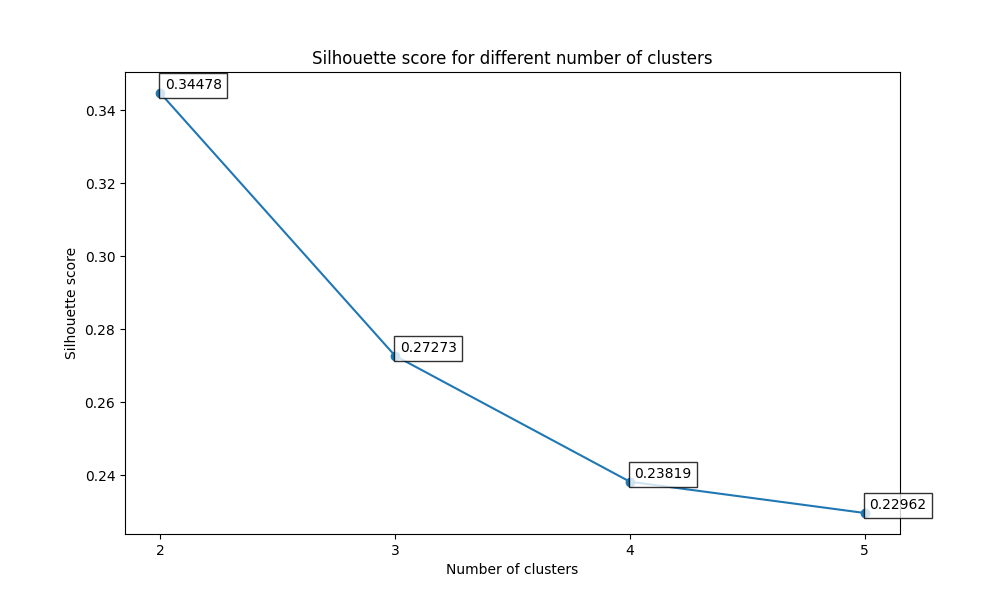
\includegraphics[width=0.8\textwidth]{images/silhouette.png}
  \caption{Silhouette score for different number of clusters}
  \label{fig:silhouette}
\end{figure}

\begin{figure}[H]
  \centering
  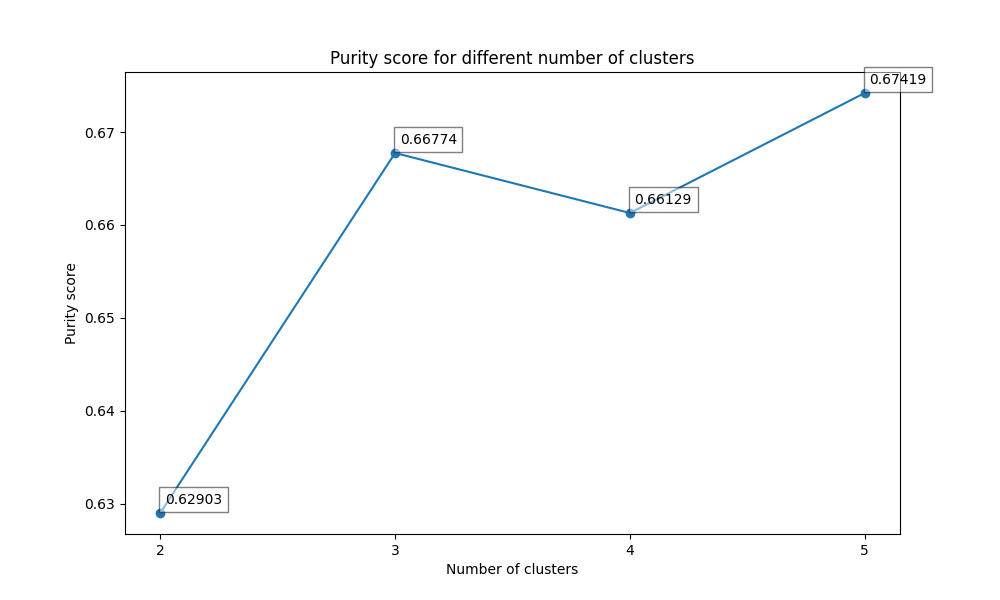
\includegraphics[width=0.8\textwidth]{images/purity.png}
  \caption{Purity score for different number of clusters}
  \label{fig:purity}
\end{figure}

\textbf{Comment}

\begin{itemize}
  \item For k=2, the silhouette score is 0.34478 and the purity score is 0.62903. Indicating that the clustering with two clusters has relatively good cohesion and separation, with data points well-matched to their own clusters and somewhat distant from other clusters. The purity score suggests that the majority of data points within each cluster belong to the same class, but there
  is some mixing of classes.
  \item For k=3, the silhouette score decreases to 0.27273, which may indicate some overlap or less distinct clusters. However, the purity score improves to 0.66774, indicating that each cluster contains a higher proportion of data points from a single class. This suggests a trade-off between silhouette and purity.
  \item For k=4, the silhouette score further decreases to 0.23819, indicating more overlap or less distinct clusters. The purity score remains relatively high at 0.66129, indicating good consistency with class labels.
  \item For k=5, the silhouette score decreases to 0.22962, indicating more overlap or less distinct clusters. The purity score remains relatively high at 0.67419, indicating good consistency with class labels.
\end{itemize}

Overall, these results show that the choice of the number of clusters (k) affects the quality of the clustering solution. A smaller k (k=2) results in better silhouette scores but lower purity, indicating that clusters are more distinct but not as pure in terms of class membership. A larger k (k=5) provides higher purity but lower silhouette scores, suggesting more class consistency but potentially less distinct clusters. The choice of k should be made based on the specific aim of the clustering task, considering the trade-off between silhouette and purity.

\subsection*{Question 2}
\begin{lstlisting}[language=Python]
  # Apply PCA to reduce the dimensionality to 2
  pca = PCA(n_components=2)
  X_pca = pca.fit_transform(X_scaled)
  
  # Plot the data
  plt.figure(figsize=(10, 6))
  plt.scatter(X_pca[:, 0], X_pca[:, 1])
  plt.xlabel('First principal component')
  plt.ylabel('Second principal component')
  plt.title('Data after PCA')
  plt.savefig(IMAGES_DIR / 'pca.png')
  plt.show()
\end{lstlisting}

\begin{figure}[H]
  \centering
  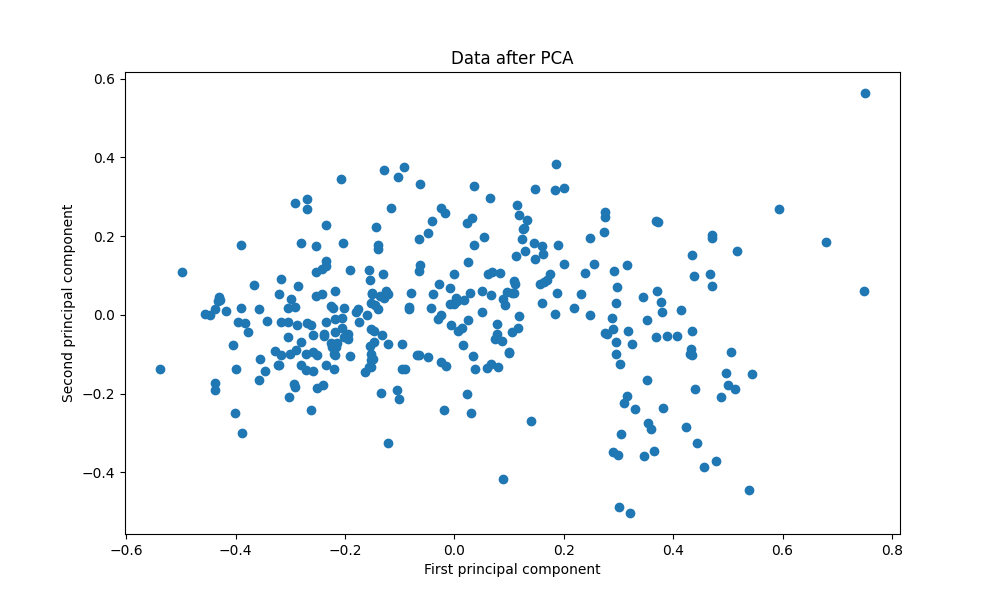
\includegraphics[width=0.8\textwidth]{images/pca.png}
  \caption{Data after PCA}
  \label{fig:pca}
\end{figure}

\textbf{i)}

\begin{lstlisting}[language=Python]
  print(f'Explained variance: {pca.explained_variance_ratio_}')
\end{lstlisting}
\begin{lstlisting}[language=Python]
Explained variance: [0.56181445 0.20955953]
\end{lstlisting}

\textbf{Comment}

When considering the variability explained by the top two principal components in a PCA (Principal Component Analysis), the values represent the proportion of total variance in the data that is captured by each of these components.
\begin{itemize}
  \item PC1 captures the largest portion of variance in the data, about 57\%. This suggests that PC1 is a significant component that summarizes the primary patterns in the data. A high value for PC1 indicates that it carries substantial information about the relationships between the original features.
  \item PC2 explains the next largest portion of variance after PC1. It captures approximately 20.96\% of the total variability. While PC2 has less explanatory power than PC1, it is still an important component that contributes significantly to the data's structure. PC2 may represent additional patterns that are orthogonal to those captured by PC1.
\end{itemize}
When summing the explained variances of PC1 and PC2 (0.56181445 + 0.20955953), you get a total explained variance of approximately 77.14%. This means that these two principal components collectively account for approximately 77.14% of the total variance in the data.

The proportion of variance explained by the top principal components informs about the dimensionality reduction achieved by the PCA. In this case, a significant amount of variability is retained by considering only the top two principal components, which can be beneficial for simplifying the data while preserving the most essential information.
However, one may need to perform a deeper analysis of the eigenvectors associated with these components to help identify which original features contribute the most to each principal component.


\textbf{ii)}

\begin{lstlisting}[language=Python]
  # Compute Column Importance for each component
  xvector = pca.components_[0] * max(X_pca[:,0])
  yvector = pca.components_[1] * max(X_pca[:,1])

  columns = X.columns
  impt_features = {columns[i] : math.sqrt(xvector[i]**2) for i in range(len(columns))}
  sorted_features = sorted(zip(impt_features.values(),impt_features.keys()),reverse=True)
  print("Features by importance for first component:\n")
  for i in range(len(sorted_features)):
      print(f'{sorted_features[i][1]} : {sorted_features[i][0]:.5f}')

  impt_features = {columns[i] : math.sqrt(yvector[i]**2) for i in range(len(columns))}
  sorted_features = sorted(zip(impt_features.values(),impt_features.keys()),reverse=True)
  print("\nFeatures by importance for second component:\n")
  for i in range(len(sorted_features)):
      print(f'{sorted_features[i][1]} : {sorted_features[i][0]:.5f}')

  # Compute Column Importance and Sort
  columns = X.columns
  impt_features = {columns[i] : math.sqrt(xvector[i]**2 + yvector[i]**2) for i in range(len(columns))}
  sorted_features = sorted(zip(impt_features.values(),impt_features.keys()),reverse=True)
  print("\nFeatures by importance:\n")
  for i in range(len(sorted_features)):
      print(f'{sorted_features[i][1]} : {sorted_features[i][0]:.5f}')
\end{lstlisting}

\begin{lstlisting}[language=Python]
  Features by importance for first component:

  pelvic_incidence : 0.44394
  lumbar_lordosis_angle : 0.38651
  pelvic_tilt : 0.35046
  sacral_slope : 0.24439
  degree_spondylolisthesis : 0.16278
  pelvic_radius : 0.08691
  
  Features by importance for second component:
  
  pelvic_tilt : 0.37797
  pelvic_radius : 0.32762
  sacral_slope : 0.24994
  pelvic_incidence : 0.05640
  lumbar_lordosis_angle : 0.04513
  degree_spondylolisthesis : 0.00258
  
  Features by importance:
  
  pelvic_tilt : 0.51544
  pelvic_incidence : 0.44751
  lumbar_lordosis_angle : 0.38913
  sacral_slope : 0.34957
  pelvic_radius : 0.33895
  degree_spondylolisthesis : 0.16280
\end{lstlisting}

\textbf{Comment}
The first principal component (PC1) is mainly influenced by features related to pelvic and lumbar angles and tilts. This suggests that PC1 might represent a combination of characteristics related to the angles and tilts of the pelvis and lumbar spine.
The second principal component (PC2) is primarily associated with pelvic tilt and pelvic radius. It may capture variations in the tilt and radius of the pelvic region.
Understanding the feature importance in each principal component can help interpret and use the components for dimensionality reduction or feature selection while preserving the most relevant information in the data.

\subsection*{Question 3}
\begin{lstlisting}[language=Python]
  # K-means clustering with k = 3
  k = 3
  kmeans = KMeans(n_clusters=k,
                  random_state=0)
  cluster_labels = kmeans.fit_predict(X_scaled)
  
  # Plot the data with y = ground truth
  target_names = y.unique()
  colors = ['navy', 'turquoise', 'darkorange']
  plt.figure(figsize=(10, 6))
  
  for i, targets in enumerate(target_names):
      plt.scatter(X_pca[y==targets,0],
                  X_pca[y==targets,1],
                  color=colors[i],
                  alpha=.8,
                  lw=2,
                  label=targets)
  
  plt.legend(loc='best', shadow=False, scatterpoints=1)
  plt.title('Points with Ground truth')
  plt.savefig(IMAGES_DIR / 'ground_truth.png')
  plt.show()
  
  # Plot the data with y = cluster labels
  plt.figure(figsize=(10, 6))
  
  
  
  for i, targets in enumerate(target_names):
      plt.scatter(X_pca[cluster_labels==i,0],
                  X_pca[cluster_labels==i,1],
                  color=colors[i],
                  alpha=.8,
                  lw=2)
  
  plt.title('Clusters for k = 3 using K-means')
  plt.savefig(IMAGES_DIR / 'clusters.png')
  plt.show()
  
  # Clusters if we assigned the max ground truth class to each cluster
  # Attribute Cluster label to a ground truth class
  clusters = {i: [] for i in range(3)}
  for i in range(len(cluster_labels)):
      clusters[cluster_labels[i]].append(y[i])
  for i in range(len(clusters)):
      print(f'cluster {i}')
      print(f'Normal: {clusters[i].count("Normal")}')
      print(f'Hernia: {clusters[i].count("Hernia")}')
      print(f'Spondylolisthesis: {clusters[i].count("Spondylolisthesis")}\n')
  lista = [max(clusters[i], key=clusters[i].count) for i in range(3)]
  print(lista)
  
  plt.figure(figsize=(10, 6))
  for i, targets in enumerate(target_names):
      plt.scatter(X_pca[cluster_labels==i,0],
                  X_pca[cluster_labels==i,1],
                  color=colors[i],
                  alpha=.8,
                  lw=2,
                  label=lista[i])
  plt.legend(loc='best', shadow=False, scatterpoints=1)
  plt.title('Clusters for k = 3 using K-means and labelled with the most frequent class')
  plt.savefig(IMAGES_DIR / 'clusters_frequency.png')
  plt.show()
\end{lstlisting}

\begin{figure}[H]
  \centering
  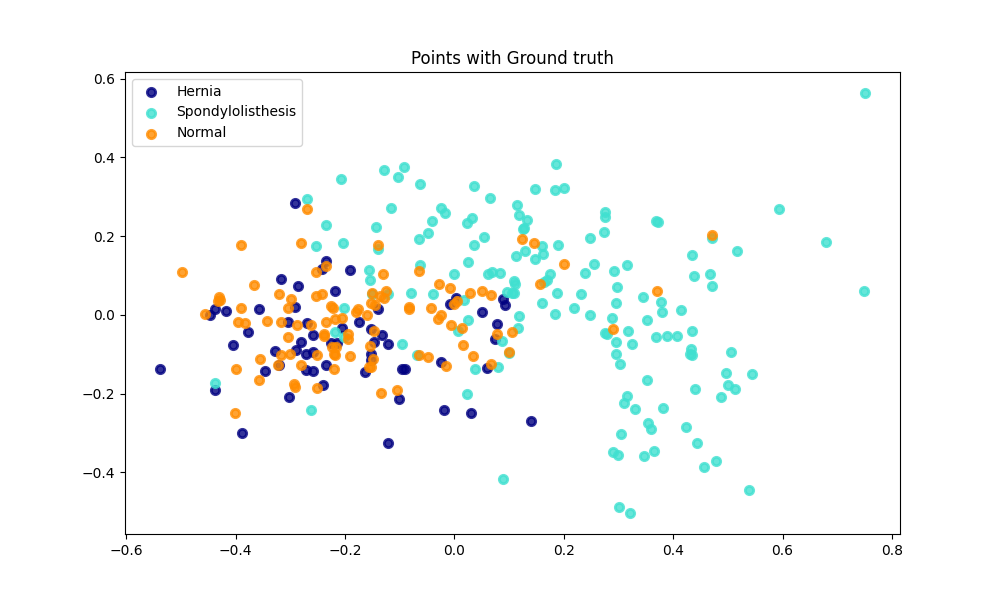
\includegraphics[width=0.8\textwidth]{images/ground_truth.png}
  \caption{Points with Ground truth}
  \label{fig:ground_truth}
\end{figure}

\begin{figure}[H]
  \centering
  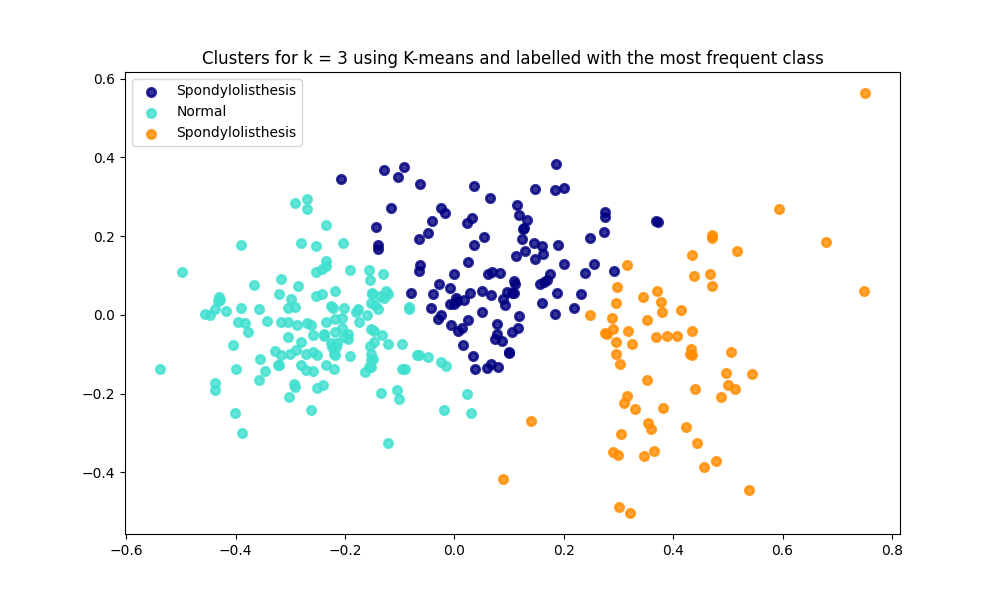
\includegraphics[width=0.8\textwidth]{images/clusters.png}
  \caption{Clusters for k = 3 using K-means}
  \label{fig:clusters}
\end{figure}

\textbf{Label the clusters with the most frequent class for visualization}

\begin{lstlisting}[language=Python]
  cluster 0
  Normal: 24
  Hernia: 8
  Spondylolisthesis: 73
  
  cluster 1
  Normal: 73
  Hernia: 51
  Spondylolisthesis: 16
  
  cluster 2
  Normal: 3
  Hernia: 1
  Spondylolisthesis: 61
  
  ['Spondylolisthesis', 'Normal', 'Spondylolisthesis']
\end{lstlisting}

\begin{figure}[H]
  \centering
  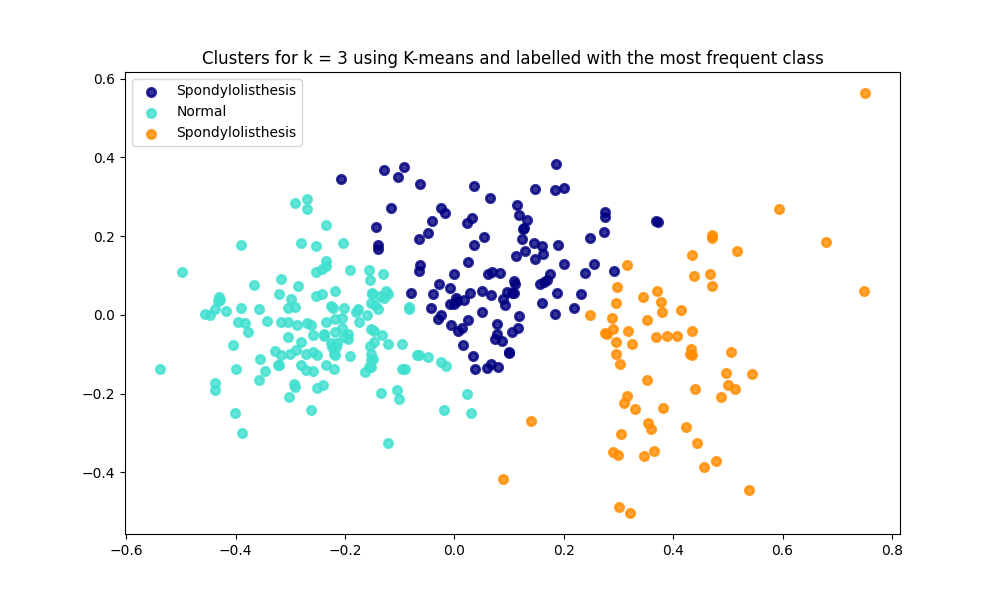
\includegraphics[width=0.8\textwidth]{images/clusters_frequency.png}
  \caption{Clusters for k = 3 using K-means and labelled with the most frequent class}
  \label{fig:clusters_frequency}
\end{figure}

\subsection*{Question 4}

Using the results we obtained for Question 1 and Question 3, we conclude that one may use clustering to identify groups of patients with similar characteristics to perform a potential diagnosis on a new patient or even to subtype groups inside a major one for specific treatments. However, one need to be careful while fine-tuning the clusters, due to the trade-off we observed between silhouette and purity scores.
In addition, one may use PCA to reduce the dimensionality of the data and identify the most relevant features for the clustering task.
However, one need to be careful while selecting the number of principal components to retain, as this may affect the amount of information retained in the data. Also, we need to be careful, since the clusters might not represent quite well the classes of the patients.
It's important to recognize that the clusters generated through clustering may not perfectly align with the known classes of patients.
For instance, in Question 3, where we plotted three clusters and have three ground truth classes, the cluster-class mapping is not straightforward, since the clusters do not represent the classes in a one-to-one fashion.
Two clusters may correspond to the same class, as we can see in the labelled clusters using the most frequent class. Suggestions for merging these clusters into one may be considered in further post-processing steps.
The third cluster, representing a mix of about 50% Normal and 50% Hernia, does not effectively represent the known classes. This incongruity can pose mistakes if used for diagnosis.
In light of these considerations, the application of clustering for diagnosis requires careful attention. While it can be a valuable tool for identifying patient groups with similar characteristics, it should be complemented with domain knowledge and a thorough understanding of the data.








\end{document}